\subsection[Ellipsoids in data space and beta space]{Ellipsoids in data space and $\vec{\beta}$ space}\label{sec:betaspace}

It is most common to look at data and fitted models in ``data space,'' where axes correspond to
variables, points represent observations, and fitted models are plotted as lines (or planes) in this space.
As we've suggested, data ellipsoids provide informative summaries of relationships in data space.
For linear models, particularly regression models with quantitative predictors, there is another space---``$\vec{\beta}$ space''---that provides deeper views of models and the relationships among them.
In $\vec{\beta}$ space, the axes pertain to coefficients and points are models (true, hypothesized, fitted) whose coordinates
represent values of parameters.

In the sense described below, data space and $\vec{\beta}$ space are \emph{dual} to each other.
In simple linear regression, for example, each line in data space corresponds to a point in $\vec{\beta}$ space,
the set of points on any line in $\vec{\beta}$ space corresponds to a pencil of lines through a given point
in data space, and the proposition that every pair of points defines a line in one space corresponds to
the proposition that every two lines intersect in a point in the other space.

Moreover, ellipsoids in these spaces are dual and inversely related to each other.
In data space, joint confidence intervals for the mean vector or joint prediction
regions for the data are given by the ellipsoids $(\bar{x}_1, \bar{x}_2)\trans \oplus c \sqrt{\mat{S}}$.
In the dual $\vec{\beta}$ space, joint confidence regions for the parameters
are given by ellipsoids of the form $\widehat{\vec{\beta}} \oplus c \sqrt{\mat{S}^{-1}}$.
We illustrate these relationships in the example below.

\begin{figure}[htb]
  \centering
  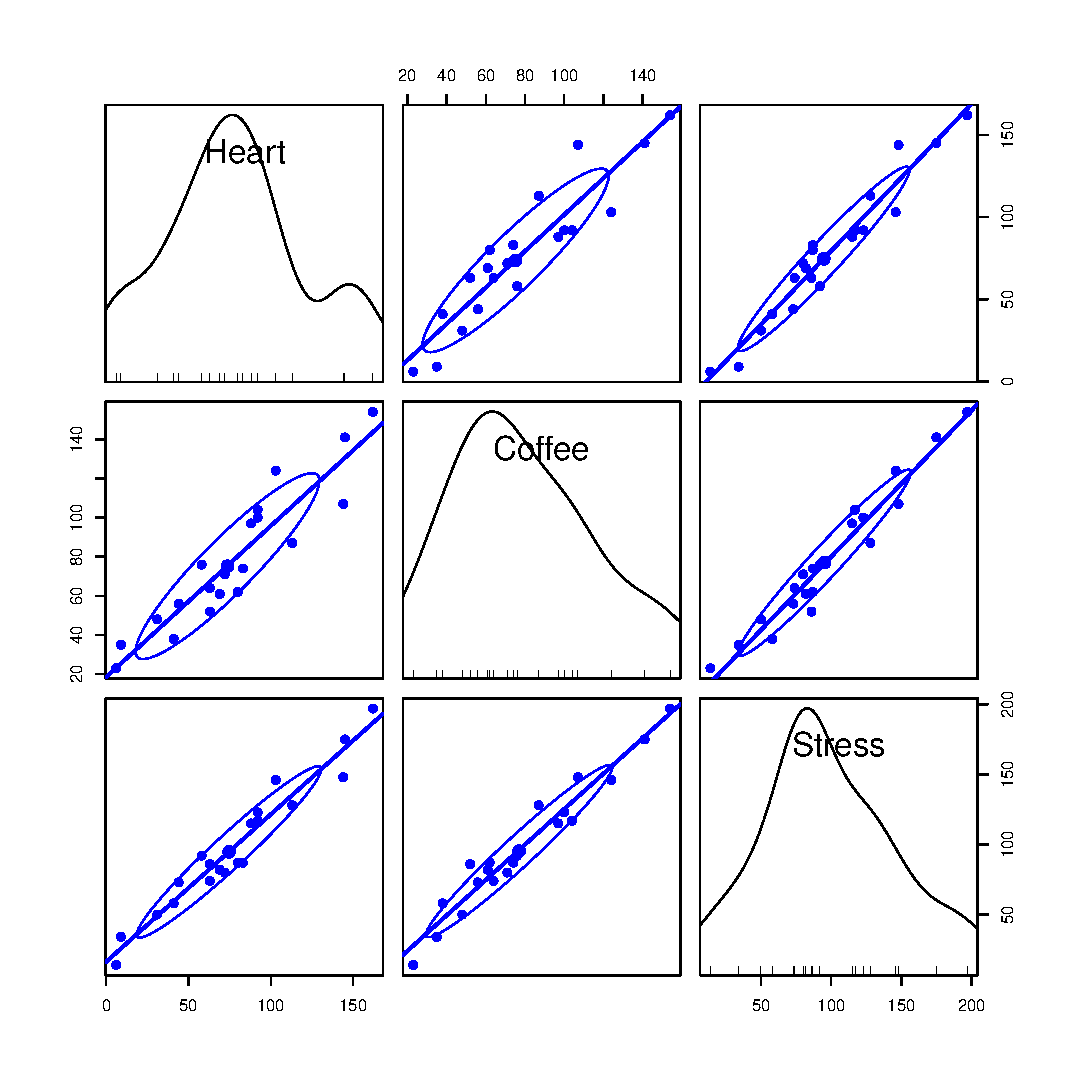
\includegraphics[width=.6\textwidth,clip]{fig/vis-reg-coffee11}
  \caption{Scatterplot matrix, showing the pairwise relationships among Heart ($y$), Coffee ($x_1$), and Stress ($x_2$),
  with linear regression lines and 68\% data ellipses for the marginal bivariate relationships.
  }%
  \label{fig:vis-reg-coffee11}
\end{figure}

\figref{fig:vis-reg-coffee11} shows a scatterplot matrix among the variables
Heart ($y$), an index of cardiac damage, Coffee ($x_1$), a measure of daily
coffee consumption, and Stress ($x_2$), a measure of occupational stress, in a contrived
sample of $n=20$. For the sake of the example we assume that the main goal is
to determine whether or not coffee is good or bad for your heart, and stress
represents one potential confounding variable among others (age, smoking, etc.)
that might be useful to control statistically.

The plot in \figref{fig:vis-reg-coffee11} shows only the marginal relationship
between each pair of variables. The marginal message seems to be that coffee is
bad for your heart, stress is bad for your heart and coffee consumption is
also related to occupational stress.
\begin{figure}[htb]
% two figs side-by-side
  \begin{minipage}[c]{.485\textwidth}
   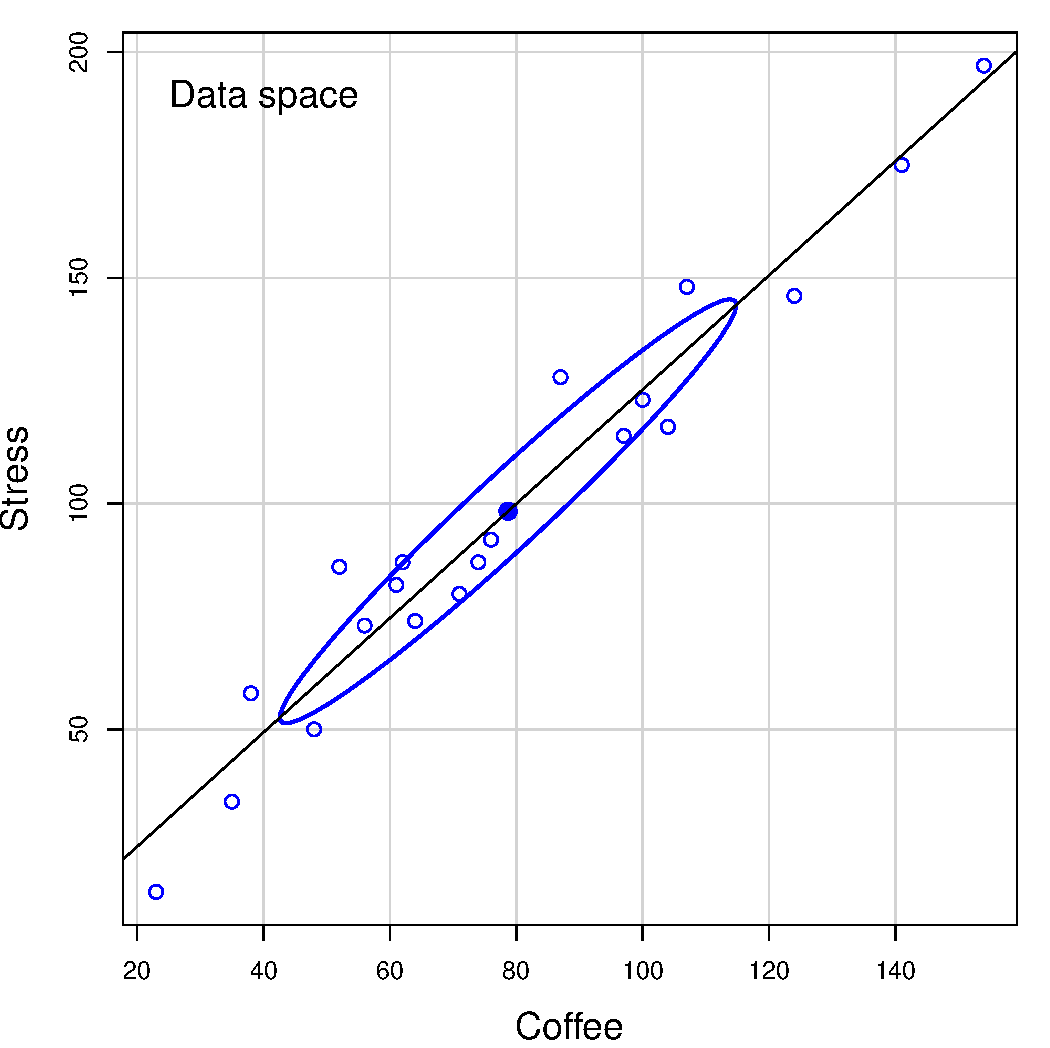
\includegraphics[width=1\linewidth,clip]{fig/vis-reg-coffee12a}
   \end{minipage}%
  \hfill
  \begin{minipage}[c]{.485\textwidth}
   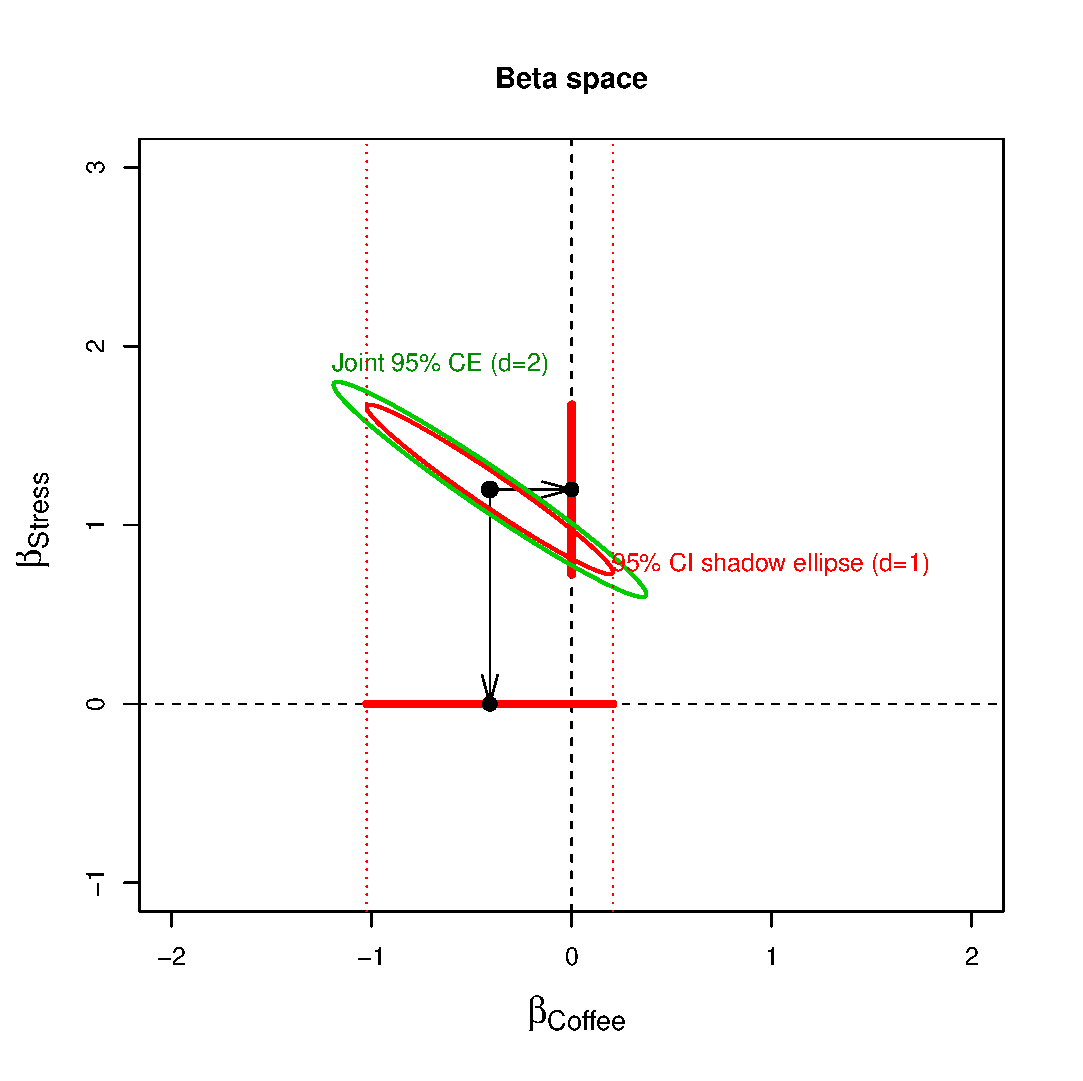
\includegraphics[width=1\linewidth,clip]{fig/vis-reg-coffee12b}
  \end{minipage}
  \caption{Data space and $\vec{\beta}$ space representations of Coffee and Stress.
   Left: Standard (40\%) data ellipse. Right: Joint 95\% confidence ellipse (green) for
   ($\beta_{\mathrm{Coffee}}, \beta_{\mathrm{Stress}}$), CI ellipse (red) with 95\% univariate shadows.
  }%
  \label{fig:vis-reg-coffee12}
\end{figure}
Yet, when we fit both variables together, we obtain the following results,
suggesting that coffee is good for you (the coefficient for coffee is now
negative, though non-significant).  How can this be?

% latex table generated in R 2.12.2 by xtable 1.5-6 package
% Fri Jun 03 09:01:43 2011
%\begin{table}[ht]
\begin{center}
\begin{tabular}{lrrrr}
%  \hline
 & Estimate ($\widehat{\beta}$) & Std. Error & $t$ value & Pr($>|t|$) \\ 
  \hline
  Intercept & -7.7943 & 5.7927 & -1.35 & 0.1961 \\ 
  Coffee & -0.4091 & 0.2918 & -1.40 & 0.1789 \\ 
  Stress & 1.1993 & 0.2244 & 5.34 & 0.0001 \\ 
   \hline
\end{tabular}
\end{center}
%\end{table}


\figref{fig:vis-reg-coffee12} shows the relationship between the
predictors in data space and how this translates into joint and
individual confidence intervals for the coefficients in
$\vec{\beta}$ space.  The left panel is the same as the corresponding
(Coffee, Stress) panel in \figref{fig:vis-reg-coffee11}, but with
a standard (40\%) data ellipse. The right panel shows the joint 95\% confidence
region and the individual 95\% confidence intervals in $\vec{\beta}$ space, determined as
\begin{equation*}
 \widehat{\vec{\beta}} \oplus \sqrt{d F^{.95}_{q, \nu}} \times s_e \times \mat{S}_X^{-1/2}
\end{equation*}
where $d$ is the number of dimensions for which we want coverage,
$\nu$ is the residual degrees of freedom for $s_e$, and $\mat{S}_X$
is the covariance matrix of the predictors.

Thus, the green ellipse in \figref{fig:vis-reg-coffee12} is the
ellipse of joint 95\% coverage, using the factor $\sqrt{2 F^{.95}_{2, \nu}}$
and covering the true values of ($\beta_{\mathrm{Stress}}, \beta_{\mathrm{Coffee}}$)
in 95\% of samples.  Moreover:
\begin{itemize*}
  \item Any \emph{joint} hypothesis (e.g., $H_0:\beta_{\mathrm{Stress}}=1, \beta_{\mathrm{Coffee}}=1$)
can be tested visually, simply by observing whether the
hypothesized point, $(1, 1)$ here, lies inside or outside the joint confidence ellipse.
  \item The shadows of this ellipse on the horizontal and vertical axes
give Scheff\'e joint 95\%  confidence intervals for the parameters, with protection for 
simultaneous inference (``fishing'')
in a 2-dimensional space.
  \item Similarly, using the factor
$\sqrt{F^{1-\alpha/d}_{1, \nu}} = t^{1-\alpha/2d}_\nu$ would give an
ellipse whose 1D shadows are $1-\alpha$ Bonferroni confidence intervals
for $d$ posterior hypotheses.
\end{itemize*}

Visual hypothesis tests and $d=1$ confidence intervals for the parameters \emph{separately}
are obtained from the red ellipse in \figref{fig:vis-reg-coffee12},
which is scaled by $\sqrt{F^{.95}_{1, \nu}} = t^{.975}_\nu$. We call this the ``confidence-interval generating ellipse'' (or, more compactly, the ``confidence-interval ellipse'').
The shadows of the confidence-interval ellipse on the axes (thick red lines) give the
corresponding individual 95\% confidence intervals, which are
equivalent to the (partial, Type III) $t$-tests for each coefficient given in the
standard multiple regression output shown above.
Thus, controlling for Stress, the confidence interval for the slope for Coffee includes 0,
so we cannot reject the hypothesis that $\beta_{\mathrm{Coffee}}=0$
in the multiple regression model, as we saw above in the numerical output.
On the other hand, the interval for the slope for Stress excludes the origin,
so we reject the null hypothesis that $\beta_{\mathrm{Stress}}=0$,
controlling for Coffee consumption.

Finally, consider the relationship between the data ellipse and the
confidence ellipse.  These have exactly the same shape, but
%(with equal coordinate scaling of the axes), 
the confidence ellipse
is exactly a $90^o$ rotation and rescaling of the data ellipse.  In directions in
data space where the data ellipse is wide---where we have more information
about the relationship between Coffee and Stress---the confidence ellipse is
narrow, reflecting greater precision of the estimates of coefficients.
Conversely, where the data ellipse is narrow (less information), the
confidence ellipse is wide (less precision). See \figref{fig:inverse}
for the underlying geometry.

\begin{figure}[htb]
  \centering
  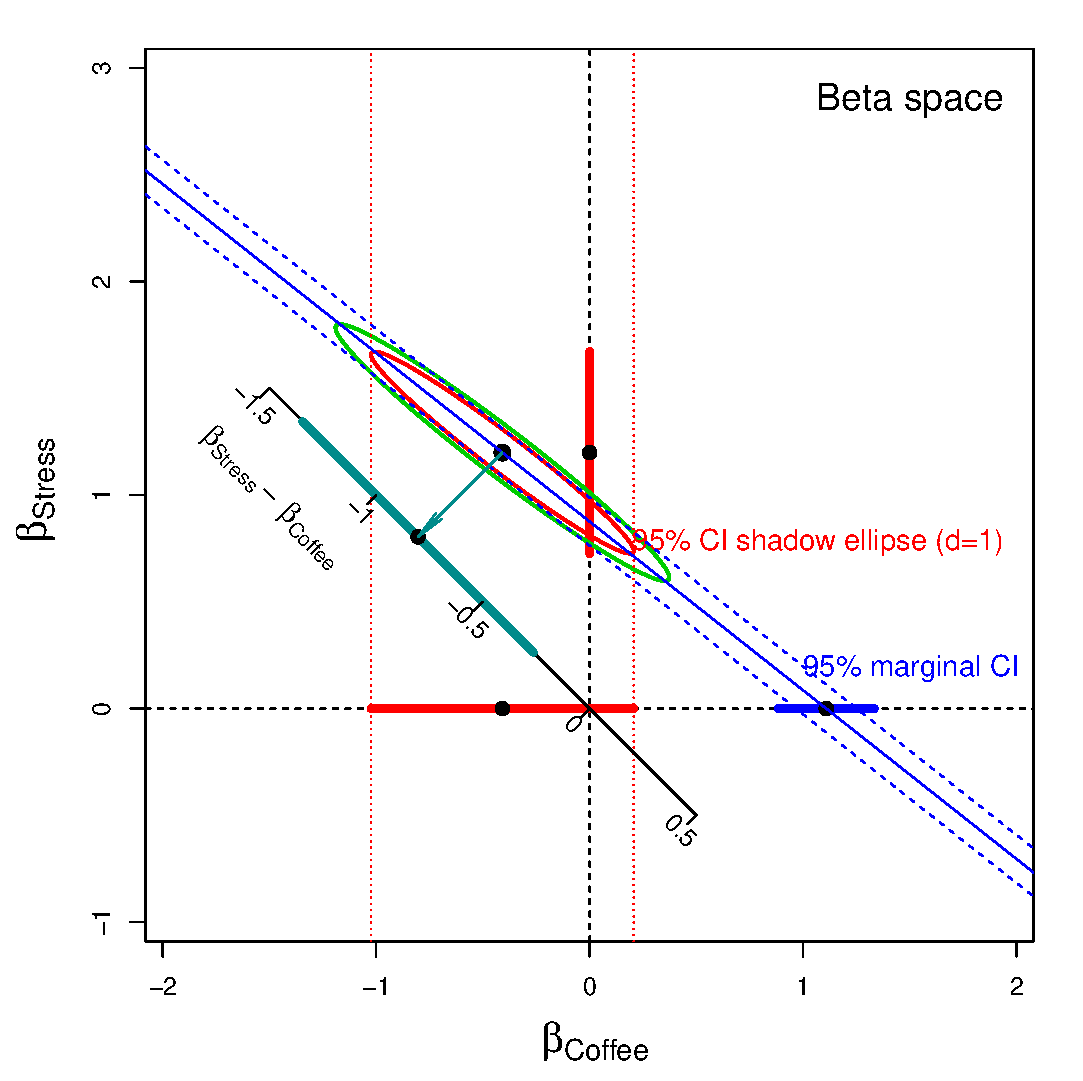
\includegraphics[width=.6\textwidth,clip]{fig/vis-reg-coffee13}
  \caption{Joint 95\% confidence ellipse for ($\beta_{\mathrm{Coffee}}, \beta_{\mathrm{Stress}}$),
  together with the 1D marginal confidence interval for $\beta_{\mathrm{Coffee}}$
  ignoring Stress (thick blue line), and a visual confidence interval for $\beta_{\mathrm{Stress}} - \beta_{\mathrm{Coffee}}=0$
  (dark cyan).
  }%
  \label{fig:vis-reg-coffee13}
\end{figure}

The virtues of the confidence ellipse for visualizing hypothesis tests and interval estimates
do not end here. Say we wanted to test the hypothesis that Coffee was unrelated to Heart damage
in the \emph{simple} regression ignoring Stress.  The (Heart, Coffee) panel in \figref{fig:vis-reg-coffee11}
showed the strong marginal relationship between the variables.  This can be seen in \figref{fig:vis-reg-coffee13} as
the oblique projection of the confidence ellipse to the horizontal axis where $\beta_{\mathrm{Stress}}=0$.
The estimated slope for Coffee in the simple regression is exactly the oblique shadow of
the center of the ellipse $(\widehat{\beta}_{\mathrm{Coffee}}, \widehat{\beta}_{\mathrm{Stress}})$
through the point where the ellipse has a horizontal tangent onto the horizontal axis at
$\beta_{\mathrm{Stress}}=0$. The thick blue line in this figure shows the confidence interval
for the slope for Coffee in the simple regression model. The confidence interval doesn't cover the origin, so
we reject $H_0:\beta_{\mathrm{Coffee}} = 0$ in the simple regression model.
The oblique shadow of the red 95\% confidence-interval ellipse onto the horizontal axis
is slightly smaller.  How much smaller is a function of the size of the coefficient for Stress.

%\begin{ADDED} %: 10-21-2011 MF
%\figref{fig:vis-reg-coffee13} has another visual interpretation in the context of \emph{mediation} models
%\citep{MacKinnon:2008}, where we are primarily interested in testing a direct, possibly causal relationship,
%$X \rightarrow Y$, but want to determine if that relation can be explained by an indirect relationship,
%$X \rightarrow M \rightarrow Y$ through a mediating $M$ variable that is correlated with both $X$ and $Y$.
%In this context, $X$ is Coffee, $Y$ is Heart damage and $M$ is Stress.
%In the figure, the significant marginal effect of Coffee ...
%\end{ADDED}

We can go further.  As we noted earlier, all linear combinations of variables or parameters
in data or models correspond graphically to projections (shadows) onto certain sub-spaces.
Let's assume that Coffee and Stress were measured on the same scales\, so it makes sense
to ask if they have equal impacts on Heart disease in the joint model that includes them both.
\figref{fig:vis-reg-coffee13} also shows an auxiliary axis through the origin with slope $=-1$
corresponding to values of $\beta_{\mathrm{Stress}} - \beta_{\mathrm{Coffee}}$. The orthogonal
projection of the coefficient vector on this axis is the point estimate of
$\widehat{\beta}_{\mathrm{Stress}} - \widehat{\beta}_{\mathrm{Coffee}}$
and the shadow of the red ellipse along this axis is the 95\% confidence interval
for the difference in slopes. This interval excludes 0, so we would reject the hypothesis
that Coffee and Stress have equal coefficients.

